\chapter{New results : Semileptonic decays of heavy mesons with artificial neural networks }\label{ANN_paper}

The study of semileptonic decays is an important new physics probe. For example, the recent analysis of semileptonic $B$ decays provides an anomaly in measurement related by lepton universality requirements. The advent of higher precision data provides new opportunities to explore whether similar anomalies exist in semileptonic decays of charmed particles \cite{Ablikim:2018evp, Ablikim:2018frk, Yuan:2019zfo, Riggio:2017zwh}.\par
Accurate theoretical description on charmed semileptonic decays provides useful information to extract the CKM matrix elements. Specifically, the decays of charmed $D^0$, $D^+$, or $D_s$ mesons provide one of the simplest way to determine the magnitudes of quark mixing parameters \cite{Grant:2019yar}. To extract these CKM matrix elements we use the knowledge of matrix elements of quark currents that describe strong interaction effects. Following from this, we find accurate description of semileptonic transitions, which is also needed for improvement of our understanding of quark hadronization mechanisms in QCD \cite{Grant:2019yar}. The exclusive semileptonnic transition between two meson states makes it a suitable system to theoretically analyze matrix elements of flavor changing currents. These flavor changing currents are parameterized by momentum dependent form factors. These form factors describes the hadronic part of the decay amplitude given by \cite{Grant:2019yar}

\begin{equation}\label{DPseudoscalar}
\langle K(\pi) (p_{K(\pi)}) | \bar q \gamma_\mu c | D (p_D) \rangle = F_+(q^2) \left(P_\mu - \frac{m_D^2-m_{K(\pi)}^2}{q^2} q_\mu \right) +
 F_0(q^2) \frac{m_D^2-m_{K(\pi)}^2}{q^2} q_\mu \ ,
\end{equation}

where $P = p_D + p_{K(\pi)}$ and $q = p_D - p_{K(\pi)}$. The differential decay rates ($d\Gamma/dq^2$) provide the means to study these form factors. By neglecting the final state fermion mass we write the differential decay rate for the semileptonic decay $D \rightarrow K(\pi) \ell \nu_{\ell}$ as \cite{Grant:2019yar}:

\begin{equation}\label{DifDistr}
\frac{d\Gamma(D \to K(\pi) \ell \nu_\ell)}{dq^2} =
\frac{G^2_F \left|V_{cq}\right|^2}{24 \pi^3} \left|{\bf p}_{K(\pi)}\right|^3 \left|F_+(q^2)\right|^2, 
\end{equation}

where $\left|{\bf p}_{K(\pi)}\right|$ is the magnitude of the $K(\pi)$ 3-momentum vector in the $D$-meson rest frame. Equation (\ref{DifDistr}) implies that only the $F_+(q^2)$ contributes for the analysis.\par  
Accurate calculations of the non-perturbative form factors $F_{+/0}(q^2)$ in the whole momentum range are very challenging \cite{Grant:2019yar}. Currently, we do not have a complete description of these form factors. Only Lattice QCD (LQCD)\cite{Aoki:2019cca} and QCD sum rules (QCDSR) \cite{Khodjamirian:2009ys} provide a model independent description in a limited $q^2$ range. However, these calculations are still improving. \par
We use rather general arguments based on analyticity of $F_+(q^2)$ to put constraints on shape of the form factors. The $z$ expansion is one of the popular approaches that uses the analyticity requirement to derive constraints on form factors. Here we series expand the form factor at some point $t=q^2$. This series can be improved by employing a conformal transformation to the parameter $z$

\begin{equation}\label{Zexp}
z(q^2)=\frac{\sqrt{t_+-t_0}-\sqrt{t_+-q^2}}{\sqrt{t_+-t_0}+\sqrt{t_+-q^2}},
\end{equation}

where the transformation $z(q^2)$ maps the interval $-\infty < q^2 < t_+$ onto the line segment $-1<z<1$. $t_0$ is a free parameter that corresponds to the values of $q^2$ that maps onto $z=0$, and $t_{\pm}= (m_D\pm m_\pi)^2$ \cite{Grant:2019yar}. Then the form factor is expanded as 

\begin{equation}\label{FF_z}
F_+(q^2)  =  \frac{1}{\Phi(q^2, t_0)} \sum_{k=0}^\infty a_k(t_0) z^k(q^2,t_0),
\end{equation}

where $\Phi(q^2, t_0)$ is an arbitrary function that is analytic anywhere but the unitarity cut \cite{Grant:2019yar,Boyd:1994tt,Becher:2005bg}. If there are poles present in between $q^2=0$ and the beginning of the unitarity cut, then the function $\Phi(q^2, t_0)$ can be written as $\Phi(q^2, t_0) = P(q^2) \phi(q^2, t_0)$, where $P(q^2) = z(q^2, m_V^2)$. For example, in $B\to \pi$ transitions such a pole present at $m_V=m_{B^*}$ \cite{Ananthanarayan:2011uc,Grinstein:2015wqa}. For the $B\to \pi$ transitions the expansion in equation (\ref{FF_z}) is converging rapidly, so only a few terms in the expansion are really needed. Thus the results from LQCD and QCDSR can be used to constrain the coefficients 
$a_k$ to provide a model-independent parameterization of the form factor \cite{Grant:2019yar}.\par
Since the form factors cannot be obtained from the first principles, phenomenological parameterizations are used to describe them. The  ``simple pole" model is the common parameterization, where ``pole'' refers to the lowest mass vector resonance formed in the t-channel with quantum numbers of the quark current \cite{Grant:2019yar}. For instance, the $D^\star$ vector state with quantum numbers $1^{-}$ is the dominant pole in the $D\to \pi e \bar\nu_e$ decay. The simple pole model is given as follows \cite{Grant:2019yar}:

\begin{equation}\label{FF_Pole}
F_+^{\rm pole}(q^2) = \frac{F_+(0)}{1-{\hat q}^2},
\end{equation}

where $F_+(0)$ is the value of the form factor at zero momentum recoil that has to be fixed either from the lattice QCD or from other arguments, and $\hat{q}^2=q^2/m_{D^*}^2$. The $m_{D*}$ is often taken as a fit parameter. However, physical masses of the states $D^*(2010)$ (for $D\to \pi$ transition) or $D^*_s(2112)$ (for $D\to K$ transition) could be used as well. Using more effective poles we construct more complicated models \cite{Grant:2019yar}

%
\begin{equation}\label{FF_ManyPoles}
F_+(q^2)=\frac{F_+(0)}{(1-\alpha)}\frac{1}{1-q^2/m_V^2}+
\sum_{k=1}^N \frac{\rho _k}{1-\frac{1}{\gamma_k}\frac{q^2}{m_V^2}},
\end{equation}

where $\alpha$  provides the strength of the dominant pole, $\rho_k$ is the strength of the $k$th term in the expansion, and
$\gamma _k=m_{V_k}^2/m_V^2$, with $m_{V_k}$ are masses of the higher mass states with vector quantum numbers. We can improve the accuracy of a given model by considering more effective poles. For example, a popular model that is due to Becirevic and Kaidalov (BK)\cite{Becirevic:1999kt} is given as 

%
\begin{equation}\label{FF_BK}
F_+^{BK}(q^2)  =  \frac{F_+(0)}{(1-\hat{q}^2)(1-a_{BK}\hat{q}^2)},
\end{equation}
%
where $a_{BK}$ is a fit parameter. 
Note that this model is obtained for the $N=1$ truncation of the expansion in equation (\ref{FF_ManyPoles}). As shown in the simple pole model, a good fit to experimental distribution is obtained 
by considering $m_V$ as a fit parameter. Further extension to the BK model is obtained by Ball and Zwicky \cite{Ball:2004ye},
%
\begin{equation}\label{FF_BZ}
F_+^{BZ} (q^2) = \frac{F_+(0)}{1-\hat{q}^2} \left(1+\frac{r_{BZ}\hat{q}^2}{1-a_{BZ}\hat{q}^2}\right),
\end{equation}
%
where $r_{BZ}$ and $a_{BZ}$ are the shape parameters.\par
In this work we are interested in learning whether choosing a specific functional form for the form factor induces a bias in the interpretation of an experimental analysis. This is analyzed in the machine learning (ML) approach. In particular, we are using the artificial neural networks (ANN) for this analysis. As shown in \cite{NNEstimator,NNEstimator2}, ANN can be used as an unbiased estimator of data. This fact has been used by the NNPDF collaboration to parameterize nucleon's parton distribution functions (PDF) \cite{Forte:2002fg,Ball:2014uwa,Rojo:2006nn}, and in form factor analysis of nucleon data \cite{Graczyk:2010gw,Alvarez-Ruso:2018rdx}.\par
In the following we build a statistical interpolating model based on ANNs, which contains information on experimental uncertainties and correlations. Nevertheless, ANN does not introduce theoretical bias. Following from \cite{Forte:2002fg,Ball:2014uwa}, we employ an approach based on multilayer feed-forward neural networks trained using the back-propagation learning algorithm \cite{Grant:2019yar}.

\section{Artificial Neural Networks}\label{ANN}
\subsection{Basic facts}

Recently, artificial neural networks are gaining traction in both academia and industry. As a result, ANN are widely used in experimental particle physics analysis. Specifically, the ANNs are extensively used in the jet finding algorithms \cite{Carleo:2019ptp}. A neural network can be thought of as a nonlinear function that connects the input and output data. In \cite{Grant:2019yar}, we explored another feature of ANNs, which is their ability to provide unbiased universal approximants to incomplete data \cite{NNEstimator,NNEstimator2}
%
\begin{center}
\begin{figure}[H]
\center
\includegraphics[scale=0.9]{Fig1.eps}
\caption{Structure of an artificial neural network with two hidden layers \cite{Grant:2019yar}. \label{Fig:ANN}}
\end{figure}
\end{center}
%
ANN mimic the structure of human neurons and consists of a set of interconnected units (see Figure.~\ref{Fig:ANN}) called {\it neurons} or {\it nodes}\cite{Grant:2019yar}. The activation state of a neuron is determined by the activation function ($g(x)$), which is determined by the activation status of the $i$ neurons connected to it. Each pair of these neurons is connected by a synapsis, which is  characterized by a weight $\omega_i$. Also, we add a threshold $\theta_i$ to control the activation state (``fire'') of neurons. In ANNs we categorize groups of neurons into layers. The first layer is called as input layer, which is associated with the input information. In the following work we used the value of $q^2$ for each bin in $q^2$ distribution of the CKM matrix element times the semileptonic form factor ($V_{cd}F_+(q^2)$) \cite{Grant:2019yar}. Furthermore, We used two nodes in the input layer, which improved the stability and the efficiency of the ANN. In section \ref{sec:feature_eng}, we provide further information on the input nodes. The final layer of the ANN is the output layer. The output layer provides fit for the $V_{cd}F_+(q^2)$ data along with its uncertainty. Conventionally, the layers between input and output layers are known as \textit{hidden layers}. Our ANN employs two hidden layers. Each of these hidden layers contain hundred nodes as well. 

\subsection{Forward propagation}
In the ANN training process we incrementally update the weights and thresholds so that they obtain optimal set of $\omega_i$ and $\theta_i$. This is achieved by minimizing the error function,
%
\begin{eqnarray}\label{error_fun}
E[{\omega,\theta}]\equiv\frac{1}{2}\sum_{A=1}^{n_p}
(o(q^2_{A})-y_{A})^2\,,
\end{eqnarray}
%
where $n_p$ is the number of pseudo-data used to train an ANN, $o( q^2_{A})$ is the output, which is given by the ANN's fit for a given input data $q^2_{A}$.
Here the target data point $y_A$, is obtained from the magnitude of the CKM matrix element times the semileptonic form factor, $\left|V_{cd} F_+(q^2)\right|$.
Note that the differential distribution of Eq.~(\ref{DifDistr}) is proportional to $\left|V_{cd} F_+(q^2)\right|^2$.
The $o(q^2_{A})$ is obtained using forward propagation. In order to achieve this we pass the input through a network of hidden nodes. The output from the first hidden layer with 
$n_1$ number of nodes is \cite{Grant:2019yar}
%
\begin{eqnarray}\label{first_layer_output}
\xi^{[1]}=g\left(\sum_{i=1}^{n_1}\omega_{i}^{[1]}q^2-\theta^{[1]}\right).
\end{eqnarray}
%
In this equation the response of each neuron is given by \cite{Grant:2019yar}
%
\begin{eqnarray}\label{sigmoid}
g(x)\equiv\frac{1}{1+e^{-x}},
\end{eqnarray}
% 
which is the \textit{sigmoid} activation function, and the summation over the $q^2$ data points is implied.
The $\xi^{[1]}$ is then used as an input for the second hidden layer with $n_2$ number of hidden nodes, and so on. The process is continued until the output layer of ANN is reached. In general, 
we can construct the output from $\ell$th hidden layer with $n_\ell$ number of nodes as \cite{Grant:2019yar}
%
\begin{eqnarray}\label{general_output}
\xi^{[\ell]}=g\left(\sum_{i=1}^{n_{\ell}}\omega_{i}^{[\ell]}\xi^{[\ell-1]}- \theta^{[\ell]} \right)  .
\end{eqnarray}
%
where $\xi^{[\ell-1]}$ is the output from the $(\ell-1)$th layer. The fit of the $L$ layer ANN $o(q^2)$ is then defined as   
%
\begin{eqnarray}
o(q^2)=\xi^{[L]}.
\end{eqnarray}
%
As shown above, the error function needed to be minimized. The popular choice of minimization is the \textit{gradient descent} (GC). Instead, 
we decided to use the non-linear conjugate gradient (NLCG) method \cite{Nocedal:2000sp, CGmethod} to minimize equation (\ref{error_fun}). 
In each iteration the $\omega_i$ and the $\theta_i$ update as \cite{Grant:2019yar}
%
\begin{eqnarray}\label{steepest_descent}
\delta\omega^{[\ell]} &=& -\eta\frac{\partial
E}{\partial\omega^{[\ell]}}\,, \nonumber \\ \\ \nonumber
\delta\theta^{[\ell]} &=& - \eta\frac{\partial
E}{\partial\theta_{i}^{[\ell]}},
\end{eqnarray} 
%
%
where $\eta$ is the learning rate at a given iteration. The NLCG method employed here does not require a pre-defined learning rate. 
The learning rate is initially determined by using line search algorithms \cite{Nocedal:2000sp}, and then iteratively updated based on the gradients that are in a conjugate direction to original gradient used in the line search algorithm. As it turns out, the NLCG method converges much faster than steepest descent method for the fits employed in this in this work. For more details on the NLCG method, see Ref. \cite{CGmethod}. 


\subsection{Back propagation}
The gradients of the error function are obtained by using the method of back propagation \cite{Demuth:2014}. 
Back propagation can be thought of as a consecutive application of the chain rule. By applying the chain rule to the $L$th layer we find \cite{Grant:2019yar}
%
\begin{eqnarray}\label{back_prop_final_layer}
\Delta^{[L]}= g'(h^{[L]})[o(q^2)-y]
\end{eqnarray} 
%
where $g'(h^{[L]})$ is the derivative of the activation function with respect to $h^{[L]}$ and 
%
\begin{eqnarray}\label{h_of_L}
h^{[L]}=\sum_{i=1}^{n_{L-1}}\omega^{[L]}\xi_{i}^{[L-1]}-\theta^{[L]}
\end{eqnarray} 
%
The derivatives with respect to $\omega_i$ and $\theta_i$ for layer $L$ are given by \cite{Grant:2019yar}
\begin{eqnarray}\label{delta}
 \frac{\partial
E}{\partial\omega_{i}^{[L]}} &=&
\Delta^{[L]}\xi_i^{[L-1]};\qquad
i=1,\ldots,n_{L-1}\,, \nonumber \\ \frac{\partial
E}{\partial\theta_{i}^{[L]}} &=& -
\Delta^{[L]}.
\end{eqnarray}
%
The output of equation (\ref{back_prop_final_layer}) is used to obtain the derivatives of the $(L-1)$th layer, $\Delta_j^{[L-1]}$,
%
\begin{eqnarray}
\Delta_j^{[L-1]}=g'\l(h^{[L-1]})
\Delta_i^{[L]}\omega^{[L]}\,.
\end{eqnarray}
%
The procedure is repeated for the hidden layers to find derivatives of error function with respect to $\omega_i$ and $\theta_i$ in each layer \cite{Grant:2019yar}, 
%
\begin{eqnarray}\label{delta1}
 \frac{\partial
E}{\partial\omega_{ij}^{[\ell]}} &=&
\Delta_i^{[\ell]}\xi_j^{[\ell-1]};\qquad
i=1,\ldots,n_\ell,\quad j=1,\ldots,n_{\ell-1}\,, \nonumber \\ 
\frac{\partial E}{\partial\theta_{i}^{[\ell]}} &=& -
\Delta_i^{[\ell]},\qquad i=1,\ldots,n_\ell,
\end{eqnarray}
%
Using these we can obtain the numerical gradient of the error function and find the corrections to the weights and thresholds. 

\section{Neural network training}
\subsection{Preparation of the data set}
The neural network training is performed on the real and artificial (pseudo) data. The pseudo data is generated based on the information from experimental data. Here we used the uncorrelated data, correlated data, normalized data, or some combination of these data types. These pseudo data was generated by following the method provided in \cite{Rojo:2006nn}. The experimental data set that is required to generate the pseudo data were provided in \cite{Ablikim:2015ixa}.
This experimental data set contains both uncorrelated and correlated statistical and systematic uncertainties. Also, the data set is provided with correlation matrices. The artificial data is generated as \cite{Grant:2019yar}
%
\begin{equation} \label{PD}
\left|V_{cd} F_{+}(q^2)\right|^{\rm{(art)},(k)}_i = \left|V_{cd} F_{+}(q^2)\right|^{\rm (exp)}_i + r_{t,i}^{(k)}\sigma_{t,i} + \sum_{j=1}^{N_{\rm sys}}r_{{\rm sys},j}^{(k)}\sigma_{{\rm sys},ji} 
+ \sum_{m=1}^{N_{\rm stat}}r_{{\rm stat},m}^{(k)}\sigma_{{\rm stat},mi}
\end{equation}
%
where $i=1,...,N_{\rm data}$ is the number of experimental data entries, which is equal to the number of $q^2$ bins. The term $\left|V_{cd} F_{+}(q^2)\right|^{\rm (exp)}_i$ is the central value of the experimental data point for a given $q^2$. The last three terms in the right hand side of the equation (\ref{PD}) provide the variation in the pseudo data sample. These terms represent total uncorrelated, correlated systematic, and correlated statistical uncertainties respectively. Following from the \cite{Rojo:2006nn}, we use all these information to generate the pseudo data samples. Here each ``uncertainty term'' is multiplied by a Gaussian random number $r_{t,i}^{(k)}$, $r_{{\rm sys},j}^{(k)}$, or $r_{{\rm stat},m}^{(k)}$  \cite{Grant:2019yar}. These random numbers have the mean of zero, and their standard deviation is equal to the bin uncertainty provided in \cite{Ablikim:2015ixa}. The total uncorrelated uncertainty, $\sigma_{t,i}$, is defined as 
%
\begin{equation}
\sigma_{t,i} = \sum_{j=1}^{N_{u,sys}}\tilde{\sigma}_{{\rm sys},ji} + \sum_{m=1}^{N_{u,sys}}\tilde{\sigma}_{{\rm stat},mi}
\end{equation}
%
where the $\tilde{\sigma}_{{\rm sys},ji}$ is uncorrelated systematic uncertainty and $\tilde{\sigma}_{{\rm stat},mi}$ statistical uncertainty. In \cite{Ablikim:2015ixa} we find the correlation matrix elements, $\mbox{corr}(j,i)$ as 
%
\begin{equation}
\sigma_{j,i} = \sqrt{\tilde{\sigma}_i \tilde{\sigma}_j \ \mbox{corr}(j,i)},
\end{equation}
%
where $\tilde{\sigma}_i$ is the uncorrelated uncertainty in the $i$-th bin of data. The $q^2$ values were randomly generated with a flat prior across the entire $q^2$ bin. Thus, every value of $d\Gamma^{\rm (art)}/dq^2$ has a different $q^2$ input. 

\subsection{Feature engineering}\label{sec:feature_eng}

We divided the generated pseudo data into 100 batches (one batch per network). Each batch has an average $q^2$ and a standard deviation relating to the $q^2$ values, which are used to scale the each value of $q^2$ which we have generated. Using the scaled $q^2$ data as a secondary input is recommended to improve the stability and the 
performance of ANNs \cite{patro2015normalization}. In particular, data standardization is a popular data scaling choice, and it is defined as 
$\tilde{q}^2_{ i\rho} = \left(q^2_{i\rho} - \bar{q}^2_{\rho}\right)/\sigma_\rho$, where $\rho$ is the batch number and $i$ is a single $q^2$ value in the batch. With this transformed data, 
each of our ANNs has the structure (2, 100, 100, 1), as the two hidden layers, each with 100 nodes, provide the most efficient structure without compromising the performance or accuracy. 
With a higher number of nodes, the ANN's fit would be more accurate, but the training speed would also be reduced. This data transformation, along with the conjugate gradient method, 
provides the minimum of the error function at $100$ iterations. In contrast, steepest descent method with a constant learning rate provides a comparable result only at 20000 iterations \cite{Grant:2019yar}. 

\section{Form factor parameterization with neural networks}

The $2\times10^{6}$ data points were generated for each of the 14 $q^2$ bins. As shown above, this data set was divided to hundred subsets, and each of these subsets contains with 280,000 unique pseudo-data points. After training all networks individually, we found the average ANN curve, with uncertainty, at every calculated $q^2$ value. The differential decay rate, $d\Gamma/dq^2$, and the $\left|V_{cd} F_{+}(q^2)\right|$ curves are shown in Fig. \ref{fig:diffGamma} and Figure \ref{fig:VFwithModels} respectively.
Further results of the ANN training and relevant graphs are available at the URL \url{https://s.wayne.edu/hepmachinelearning/}.

%

\begin{figure}[H]
\begin{center}
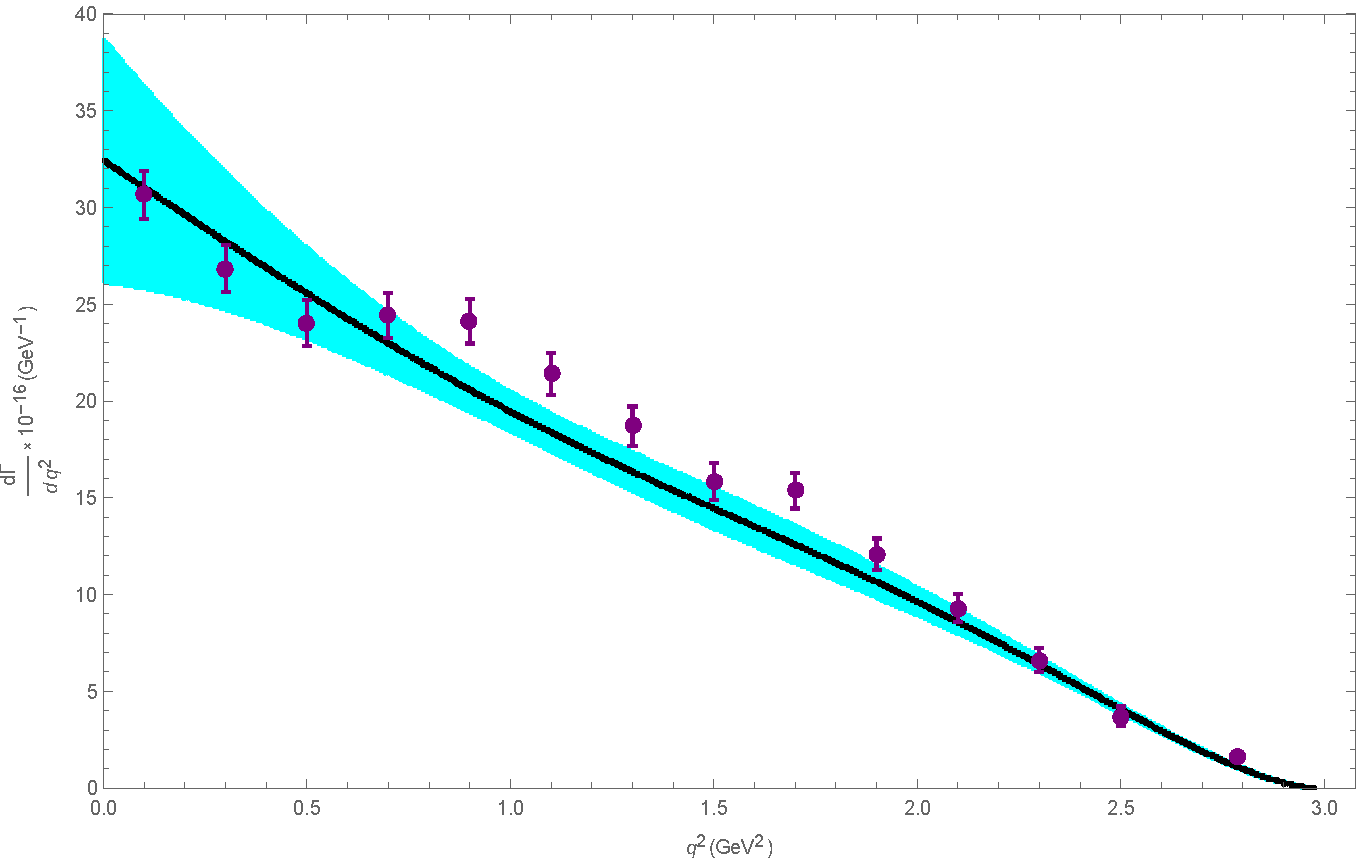
\includegraphics[scale=0.4]{FF exp final PDisVF_NN.pdf}
\caption{The averaged ANN result for the differential decay rate plotted against the experimental measurement \cite{Grant:2019yar}. The purple data points are the experimental data from \cite{Ablikim:2015ixa}. 
The black and cyan curves are the average value and one standard deviation, respectively, from the output of our averaged ANN .}
\label{fig:diffGamma}
\end{center}
\end{figure}
\vspace{-10mm}
In figure \ref{fig:VFwithModels} ANN fit is compared with some common form factor models: simple pole, the BK model (or modified pole), and the BZ model \cite{Becirevic:1999kt, Ball:2004ye} . 
%

\begin{figure}[H]
\begin{center}
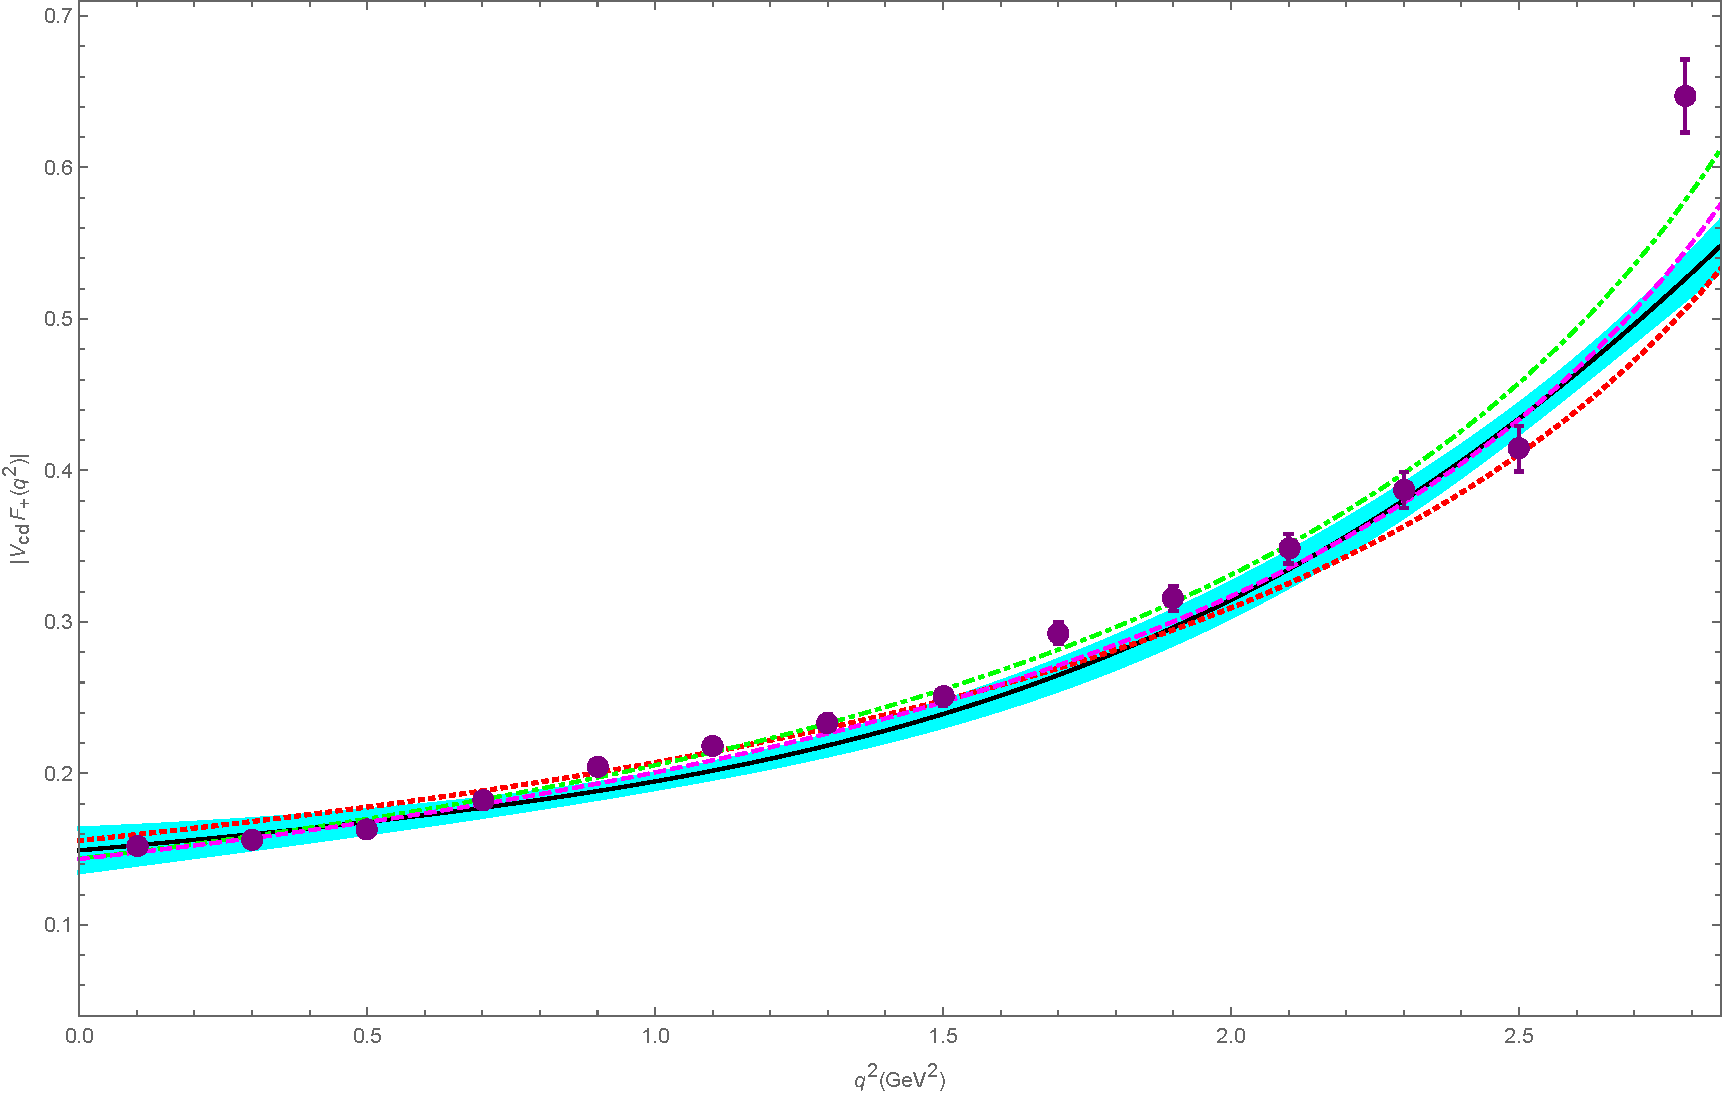
\includegraphics[scale=0.4]{FF exp final PDisVF_model.pdf}
\caption{ANN fits for $\left|V_{cd} F_+ (q^2)\right|$ plotted against the three models described in the text \cite{Grant:2019yar}. The black and cyan curves are the average value and one 
standard deviation, respectively, from the output of our neural network. The dotted red curve is the simple pole model. The dot-dashed green curve is the modified 
pole model. The dashed magenta curve is the BZ model. The purple data points are calculated from the experimental data in Ref \cite{Ablikim:2015ixa}.}
\label{fig:VFwithModels}
\end{center}
\end{figure}
\vspace{-8mm}
The $|V_{cd}F_+(0)|$ obtained from the model fits are roughly consistent with the ANN fit of the semileptonic decay data. 
%